\documentclass{sig-alternate-10pt}

\newcommand{\ttt}{\texttt}

\usepackage{graphicx}

\title{Discovery of the Higgs Boson:\\ A Social Analysis}
\author{
	Chae Jubb and Patrick Facheris \\
	\ttt{\{ecj2122,plf2110\}@columbia.edu}
}
\date{23 December 2014}

\begin{document}
\maketitle

\section{Problem Statement}
%Par. 1 general motivation, why is that pb area important
Finding reliable information on the internet is important, especially during crisis and times of extreme innovation.
In its microblogging form, Twitter provides quick access to information that anyone can post.
We can approximate the spread of this information by finding the key influencers on this platform.
For various reasons, certain individuals become a rallying point or a key participant in the spread of information.
Because a few people will dominate the information sphere, identifying these people is important.
Having this information, the media and press might target this group or a scientist might analyze it.

%Par. 2~3 narrow down: specify what choices you make and important assumptions (without being too technical)
% Hubs and authorities; SVM
We begin with the assumption that prominent events on Twitter will result in a network of similar structure to our dataset. Additionally, we assume that knowledge of auxiliary relationships between a subset of participating Twitter users will be easier to acquire than follower counts for all participating users.
We can make use of auxiliary relationships between Twitter users to extract those users providing information to the most other users.
We define these users of interest in our dataset as those with the most followers, thus most likely to convey information.
We predict users who are most responsible for providing information to the network and compare our prediction to the complete social graph ranked by number of followers.

We focus on three auxiliary data sets: retweets, replies, and mentions.
These data sets serve three distinct purposes.
\begin{description}
\item [Retweets]
    We assume this to be an indicator of a very weak relationship.
    It often serves simply as an acknowledgment of another's communication.
\item [Replies]
    Of the three, replies indicate the most direct and personal form of interaction between two users.
    We assume this to be an indicator of a tight relationship, especially if the communication is two-way.
\item [Mentions]
    Mentions are the least straightforward because their use ranges the most widely.
    It could be an invitation for communication or simply equivalent to the CC line on an email.
\end{description}
Through appropriate analysis and synthesis, we attempt to reconstruct the social graph using these auxiliary data sets.

%Par. 4 first sentence should describe your problem formulation and contribution. Typically people start this paragraph with “In this paper, we ...”
In this paper, we attempt to reconstruct a directed social network using auxiliary data concerning interactions on that network.
We focus on the spread of information surrounding the time period of the announcement of the discovery of a particle with properties similar to those of the theoretical Higgs Boson.
Our target is to extract the nodes of highest incoming degree from the social graph, indicating these users have the most followers.
Using a weighted variation of the hubs and authorities algorithm, we consider the known auxiliary data sets and calculate the hubs and authorities vector for each relationship graph.
We then take some significantly small proportion of the entire social graph relative to the number of influencer nodes we wish to identify and use these known values to train a Support Vector Machine for purposes of regression, using the hub and authority values for each graph as features.
By appropriate weighting and training, we strive to partially reconstruct the social network in question.


\section{Related Work}
% [3] Gibson: Link topology: HITS; Hubs and Authorities; importance of each, etc
% [4] Java: Hubs and Authorities on follower interaction; "User Intention": knowledge-{sharing, taking}, friendship relations.  Communities of people
% [1] Murthy: Analysis of different types of media (and authority vs. non-authority) in Pakastani flood crisis.  Legitimizes even conducting our analysis
% [2] Letierce: Analysis of Scientific Community's use of Twitter in general

We see previous authors studying the use of social network during crisis and disaster situations.
In [1], we see an analysis of the Pakastani flood crisis and the resulting Twitter use.
The focus in this research, though not important to us here, is the distribution of types of links Tweeted.
This premise of this study, that people take to Twitter (and similar social media) during crisis, legitimizes our problem area.
Moving forward from that research, we plan to investigate the structure of this news spread.

Another background source shows an analysis of the scientific community's use of Twitter to spread information---but in a general way.
A claim is made that those acting as authorities on Twitter (within the scientific community) will in general be the same group of people with the authoritative research.[2]
We use this claim as the basis for our problem exploration.
By identifying those users who are Twitter authorities (through means explained below), we can gain a sense of the scientific authorities.
Our addition to that research is our methods for gaining those authorities.

We now move to research more relevant to our specific method.
In 1998, Kleinberg, et al. give a method for describing the link topology of a network: their HITS algorithm [3].
He defines hubs and authorities as those pages with valuable links and those pages with valuable content, respectively.
We, like many others [4], are extending this hubs and authorities algorithm from an analysis of webpages to an analysis designed to determine ``authorities'' in a specific Twitter community.

Lastly, we note a specific, fantastic use of hubs and authorities when analyzing Twitter.
Java, et. al. [4], use hubs and authorities to construct communities of people.
In his communities, there may be three main types of users: knowledge-sharing, knowledge-taking, and friends.
This classification is determined by the type and frequency of interactions such as replying and retweeting.
We extend this notion of the importance of replying, retweeting, and mentioning by attempting to discern the underlying social graph using only these three types of interaction.
We attempt to apply the hubs and authorities algorithm to a graph of these interactions in order to discern a picture of the underlying follower-followee social graph.


\section{Results}
A goal N value and known N value were decided for each calculation of the precision, with the known N value varied as $.1*N$ and $.25*N$ to simulate a reasonable sampling of the known social data set.
Features of the training and testing data were determined by use of the Hubs and Authorities algorithm for each auxiliary data set and were normalized across each feature space.
This method allows us to determine those users with authority of information and predict the expected number of followers in the social graph in many varied settings.
For each run, the training set for the SVM was randomized and optimal parameters for each SVM kernel were calculated.
Predicted follower numbers sorted to decide the top N nodes and the number of nodes in the prediction was compared to the top N ranked by followers in the complete social graph.
A power model was fit to the final output of the precision data as it varied with N.
Graphs may be found in the Supplementary Information section.
\begin{description}
    \item [Claim 1.]
    \textbf{With reasonable precision we are able to predict the users with the top N followers of sufficiently large N in the social graph from auxiliary information using our method.}
    Figure~\ref{rbf_hub} shows the general trend observed in each data set as N was varied from 100 to 10000.
    For small $N \leq 1000$, we see that for most kernel test cases the precision of the estimation of the top N nodes grows significantly as N increases, plateauing at a precision of approximately $.35$.
    We determine that such an estimate is reasonable with a general trend of a decreasing error bound in these measurements.
    

    \item [Claim 2.]
    \textbf{Support vector machines used for regression were optimized for three possible kernel choices and compared, with RBF performing best.}
     A linear, radial basis function (RBF), and polynomial kernel were used with the normalized HITS scores calculated for each node from the replies, mentions, and retweets auxiliary graphs respectively as features.
     For the linear and RBF kernels, the penalty parameter of the error term was varied from $.01$ to $10000$ logarithmically and for the polynomial kernel form degree 2 to 5.
     Additionally, for the RBF kernel the gamma (kernel coefficient) parameter was varied from $1$ to $.00001$.
     Traditional cross validation techniques were used with combinations of these values to determine the optimal parameters for a given N, selecting a subset of the input training data for validation purposes.
     These optimized parameters were then used for each following run on the full testing set used for final precision calculation.
     RBF performed best for training data sized $.1*N$ and $.25*N$ for most N, with both coefficient of determination for fitting with power models closest to $1.0$.
    

    \item [Claim 3.]
    \textbf{It was found that including the hub value for a node in the regression features had no observable effect on the precision.}
    Observation of the precision graphs generated by the same kernel show a negligible effect with the inclusion of the hub values as a feature.
    (Figure~\ref{rbf_hub} and Figure~\ref{rbf_no_hub} exhibit this behavior most clearly.)
    This is expected as the hub values would likely be inversely correlated with the authority values and would not affect regression.
    
    \item [Claim 4.]
    \textbf{For the RBF kernel, there was an observable correlation between the size of the training data relative to the goal N and the precision.}
    Significant difference is observed in the power model fit for the RBF kernel with hubs.
    As N increases, both values tend to converge to approximately $.35$ with the initial difference in precision being much greater.
    The coefficient of determination for the lower training sample size indicates that the stability of these measures seems correlated with the size of the training sample, as a larger training sample allows for a better representation of the full data set.
\end{description}



\clearpage
\section{Supplementary Information}
\subsection{References}
\begin{enumerate}
\item D. Murthy, S. A. Longwell (2013) TWITTER AND DISASTERS, Information, Communications \& Society, 16:6, 837-855, DOI: 10.1080/1369118X.2012.696123

\item J. Letierce, et. al. Understanding How Twitter is Used to Spread Scientific Messages. Proceedings of the WebSci10: Extending the Frontiers of Society On-Line, April 26-27th, 2010, Raleigh, NC: US.

\item D. Gibson, J. Kleinberg, P. Raghavan.  Inferring Web Communities from Link Topology.  ACM Journal. 1998.

\item A. Java, et. al. Why We Twitter: Understanding Microblogging Usage and Communities. Joint 9th WEBKDD and 1st SNA-KDD Workshop ’07, August 12, 2007,
San Jose, California, USA
\end{enumerate}

\begin{figure}
\begin{center}
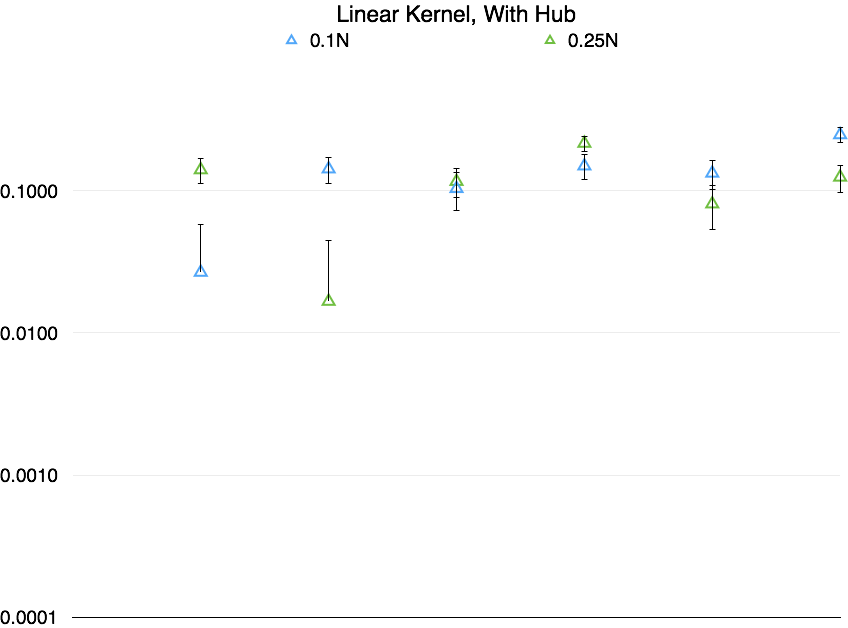
\includegraphics[width=\columnwidth]{img/linear_hub}
\caption{SVM with linear kernel considering Hubs.  We predict the top $N$ authorities (users with incoming connections) using two different proportional training sets.  The N values selected include $\{100, 200, 500, 1000, 2000, 5000, 10000, 20000, 50000\}$ from our data set of size 456631 nodes.}
\label{linear_hub}
\end{center}
\end{figure}

\begin{figure}
\begin{center}
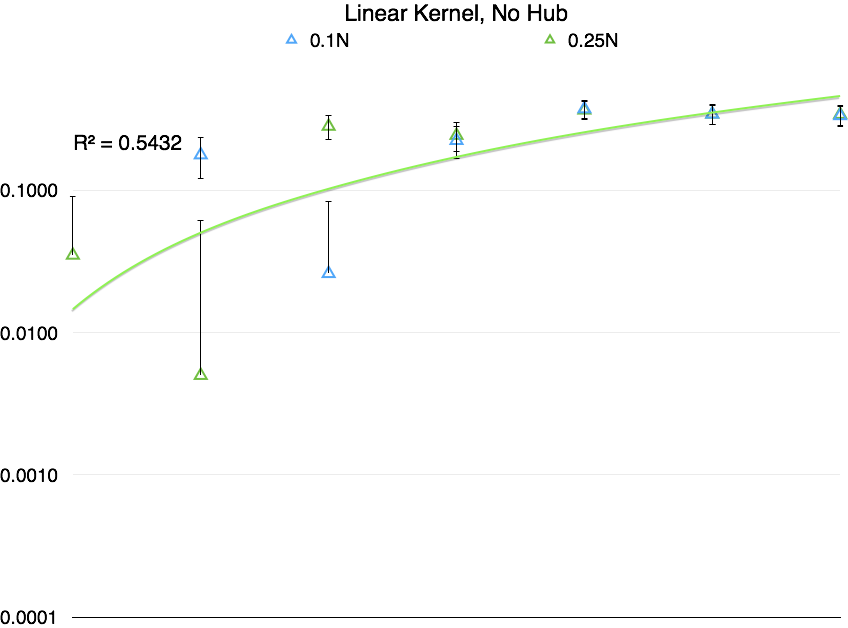
\includegraphics[width=\columnwidth]{img/linear_no_hub}
\caption{SVM with linear kernel not considering Hubs}
\label{linear_no_hub}
\end{center}
\end{figure}

\begin{figure}
\begin{center}
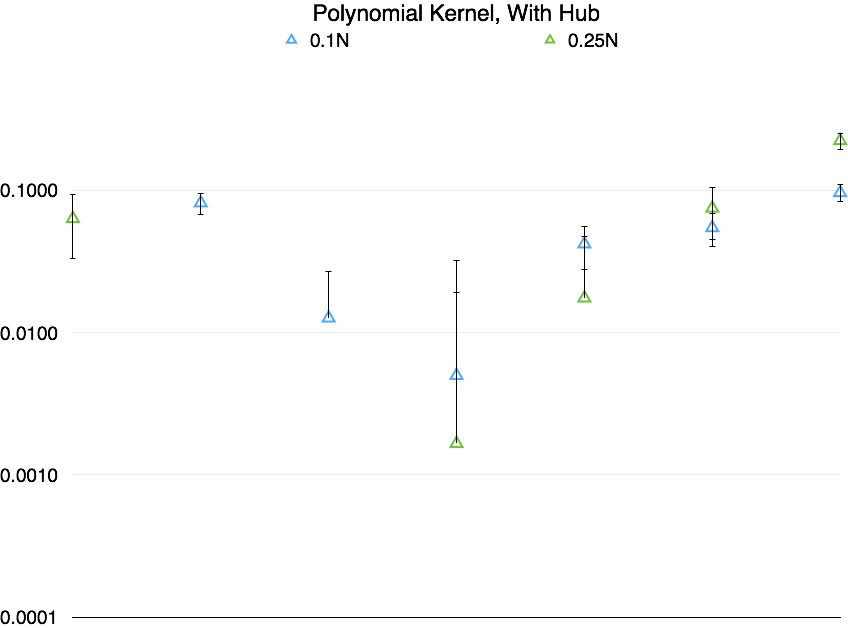
\includegraphics[width=\columnwidth]{img/poly_hub}
\caption{SVM with polynomial kernel considering Hubs}
\label{poly_hub}
\end{center}
\end{figure}

\begin{figure}
\begin{center}
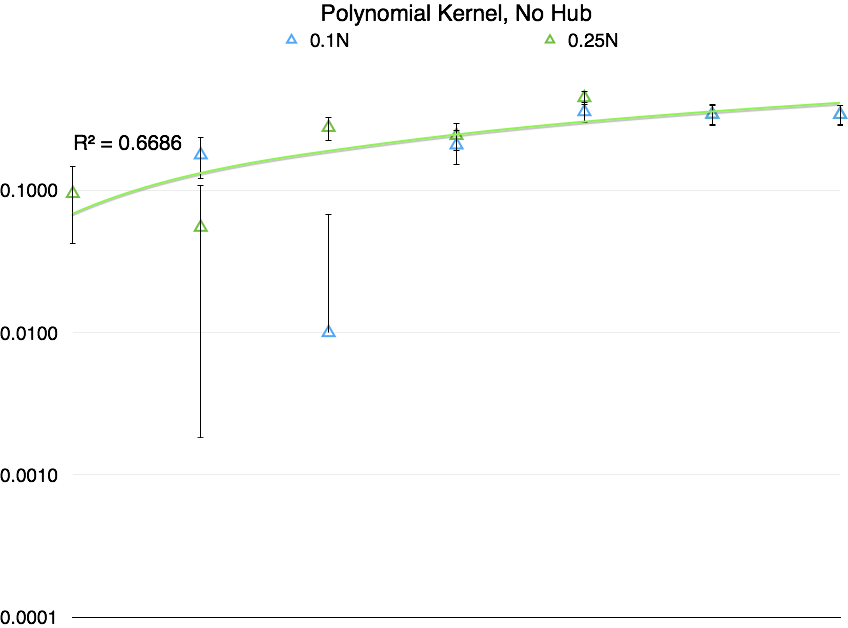
\includegraphics[width=\columnwidth]{img/poly_no_hub}
\caption{SVM with polynomial kernel not considering Hubs}
\label{poly_no_hub}
\end{center}
\end{figure}

\begin{figure}
\begin{center}
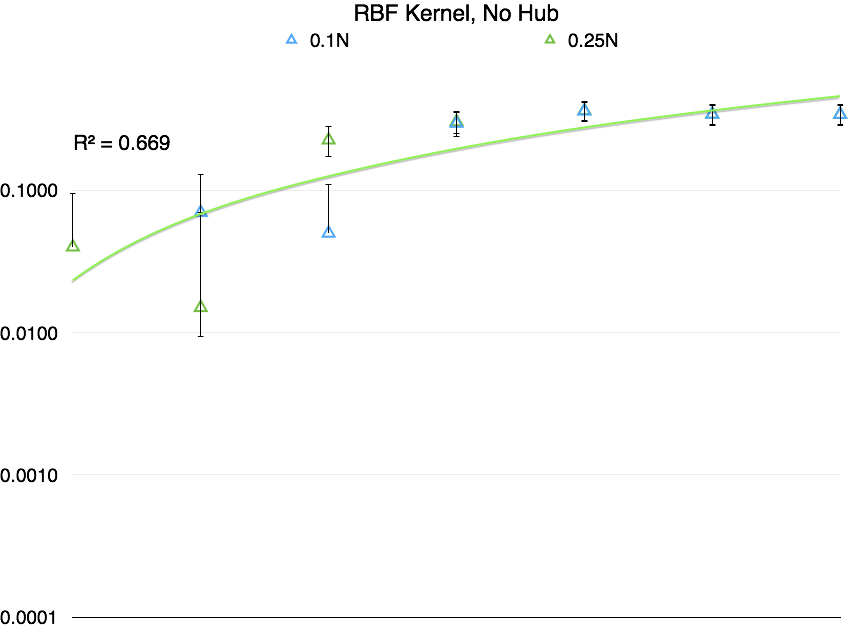
\includegraphics[width=\columnwidth]{img/rbf_no_hub}
\caption{SVM with rbf kernel considering Hubs}
\label{rbf_hub}
\end{center}
\end{figure}

\begin{figure}
\begin{center}
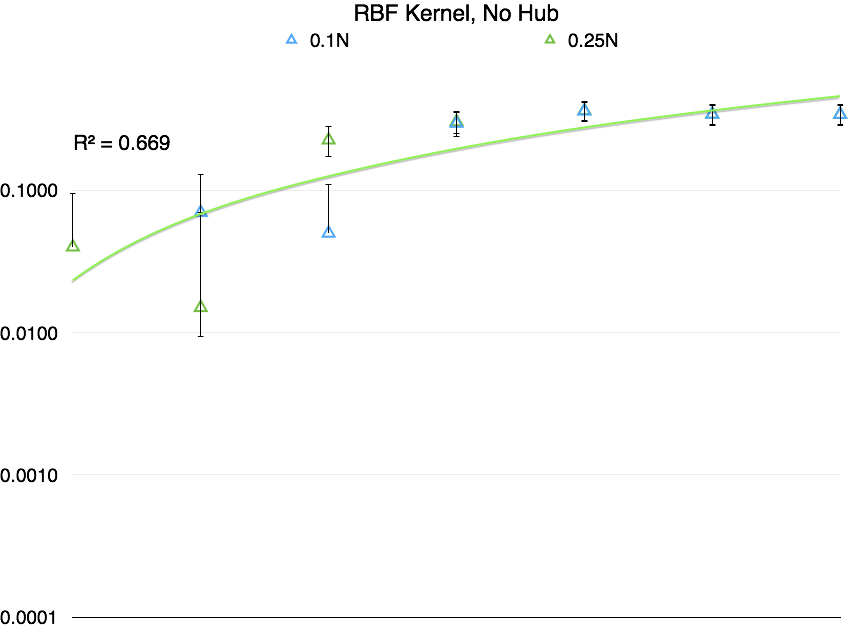
\includegraphics[width=\columnwidth]{img/rbf_no_hub}
\caption{SVM with rbf kernel not considering Hubs}
\label{rbf_no_hub}
\end{center}
\end{figure}



\end{document}
